\chapter{VAEs}
\label{chap:VAE}

% \label{sec:vae_framework}

Variational Autoencoders (VAE) learns model a complex data distribution $p(\mathbf{x})$ by assuming it is governed by unobserved, low-dimensional latent variables $\mathbf{z}$. 

\subsection{The Probabilistic Generative Process}
Once we have a trained (learned) VAE model images $\mathbf{x}$ can be generated from a latent representation $\mathbf{z}$ drawn from a prior distribution. Which is defined as :
\begin{equation} 
p_\theta(\mathbf{x}, \mathbf{z}) = p_\theta(\mathbf{x} \mid \mathbf{z}) p(\mathbf{z}) 
\end{equation} 
where $p(\mathbf{z}) \sim \mathcal{N}(0, I)$ acts as our starting point—i.e we sample from a gaussian (Normal) distribution. The decoder $p_\theta(\mathbf{x} \mid \mathbf{z})$ then decodes these samples into the high-dimensional image space.

\subsection{Variational Approximation}
In practice, identifying which latent code $\mathbf{z}$ produced a specific image $\mathbf{x}$ is computationally impossible because the true posterior $p_\theta(\mathbf{z} \mid \mathbf{x})$ is intractable. To resolve this, we introduce a secondary network—the encoder—to approximate this relationship:
\begin{equation} 
q_\phi(\mathbf{z} \mid \mathbf{x}) \approx p_\theta(\mathbf{z} \mid \mathbf{x}) 
\end{equation}
This allows us to treat the generation problem as a task of optimization rather than direct integration.

\subsection{Evidence Lower Bound : ELBO}
To train both the encoder and decoder simultaneously, we derive the Evidence Lower Bound (ELBO). This objective ensures that the model remains faithful to the original data while respecting the geometry of our latent space:
\begin{equation} 
\mathcal{L}(\theta, \phi; \mathbf{x}) = \underbrace{\mathbb{E}_{q_\phi(\mathbf{z} \mid \mathbf{x})} [\log p_\theta(\mathbf{x} \mid \mathbf{z})]}_{\text{Reconstruction Fidelity}} - \underbrace{D_{KL}(q_\phi(\mathbf{z} \mid \mathbf{x}) \| p(\mathbf{z}))}_{\text{Latent Regularization}} 
\end{equation}



% \subsection{Limitations of VAEs}

% While VAEs enable generative modeling, they exhibit several limitations:

% \begin{enumerate}
%     \item \textbf{Over-Regularized Latent Space:}  
%     The KL term forces latent encodings toward a unimodal Gaussian prior, which may suppress meaningful clustering structure in complex datasets such as chest X-rays.

%     \item \textbf{Blurry Reconstructions:}  
%     When using Gaussian likelihood assumptions, the decoder optimizes pixel-wise reconstruction loss, often leading to blurry outputs.

%     \item \textbf{Posterior Collapse:}  
%     The encoder may ignore the latent variable if the decoder is sufficiently powerful.

%     \item \textbf{Poor Class Separability:}  
%     In medical datasets with subtle pathology variations, enforcing a global Gaussian structure can mix pathological and non-pathological samples in latent space.
% \end{enumerate}



\section{Latent space visualization of VAE trained on all pathologies}
\begin{figure}[ht]
    \centering
    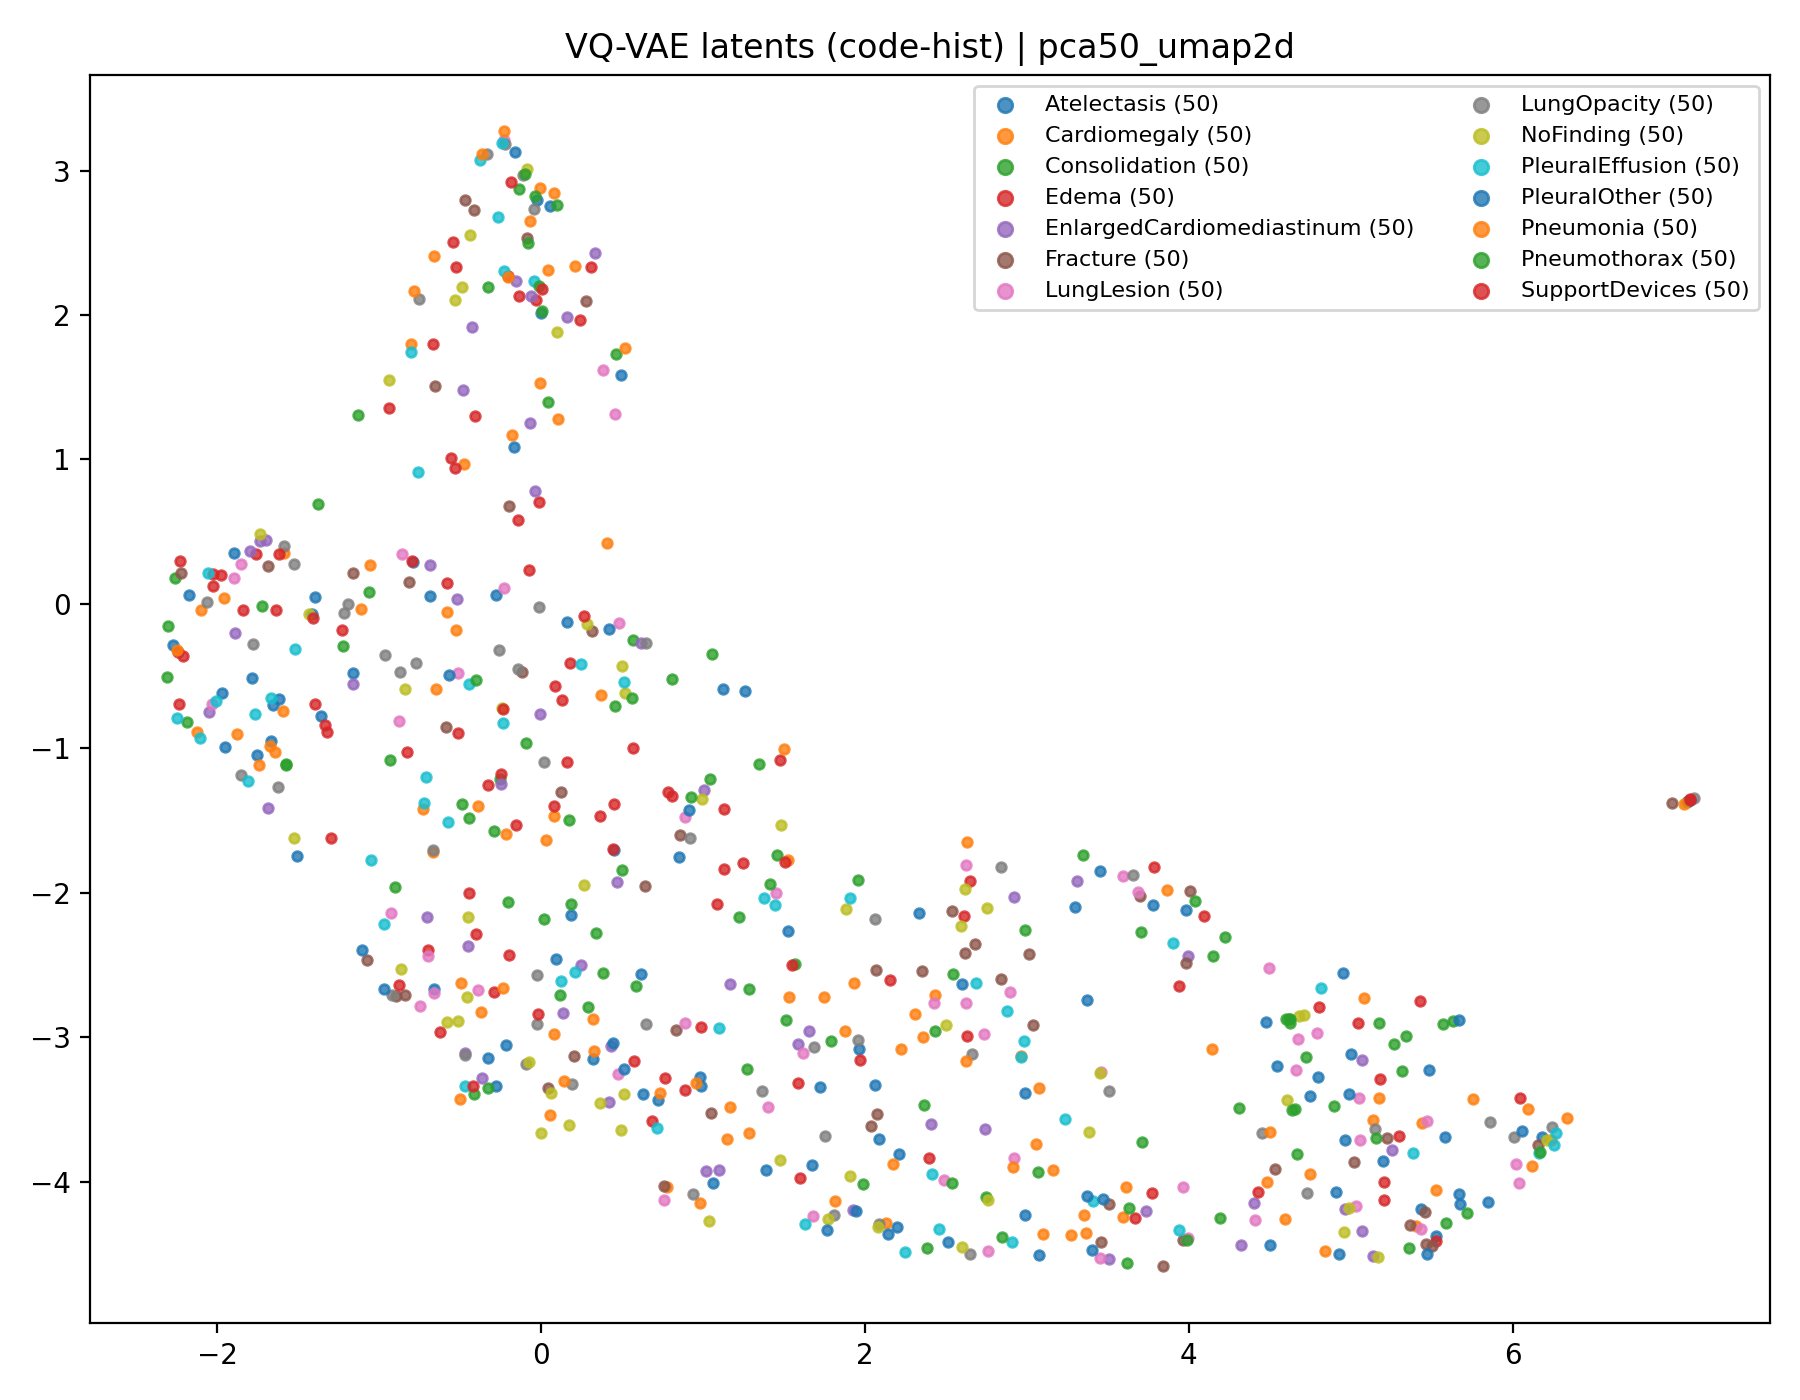
\includegraphics[width=0.8\textwidth]{./images/scatter_all_classes__pca50_umap2d.png}
    \caption{Latent space visualization of VAE trained on all pathologies.}
    \label{fig:latent_space_all}
\end{figure}

\begin{figure}[ht]
    \centering
    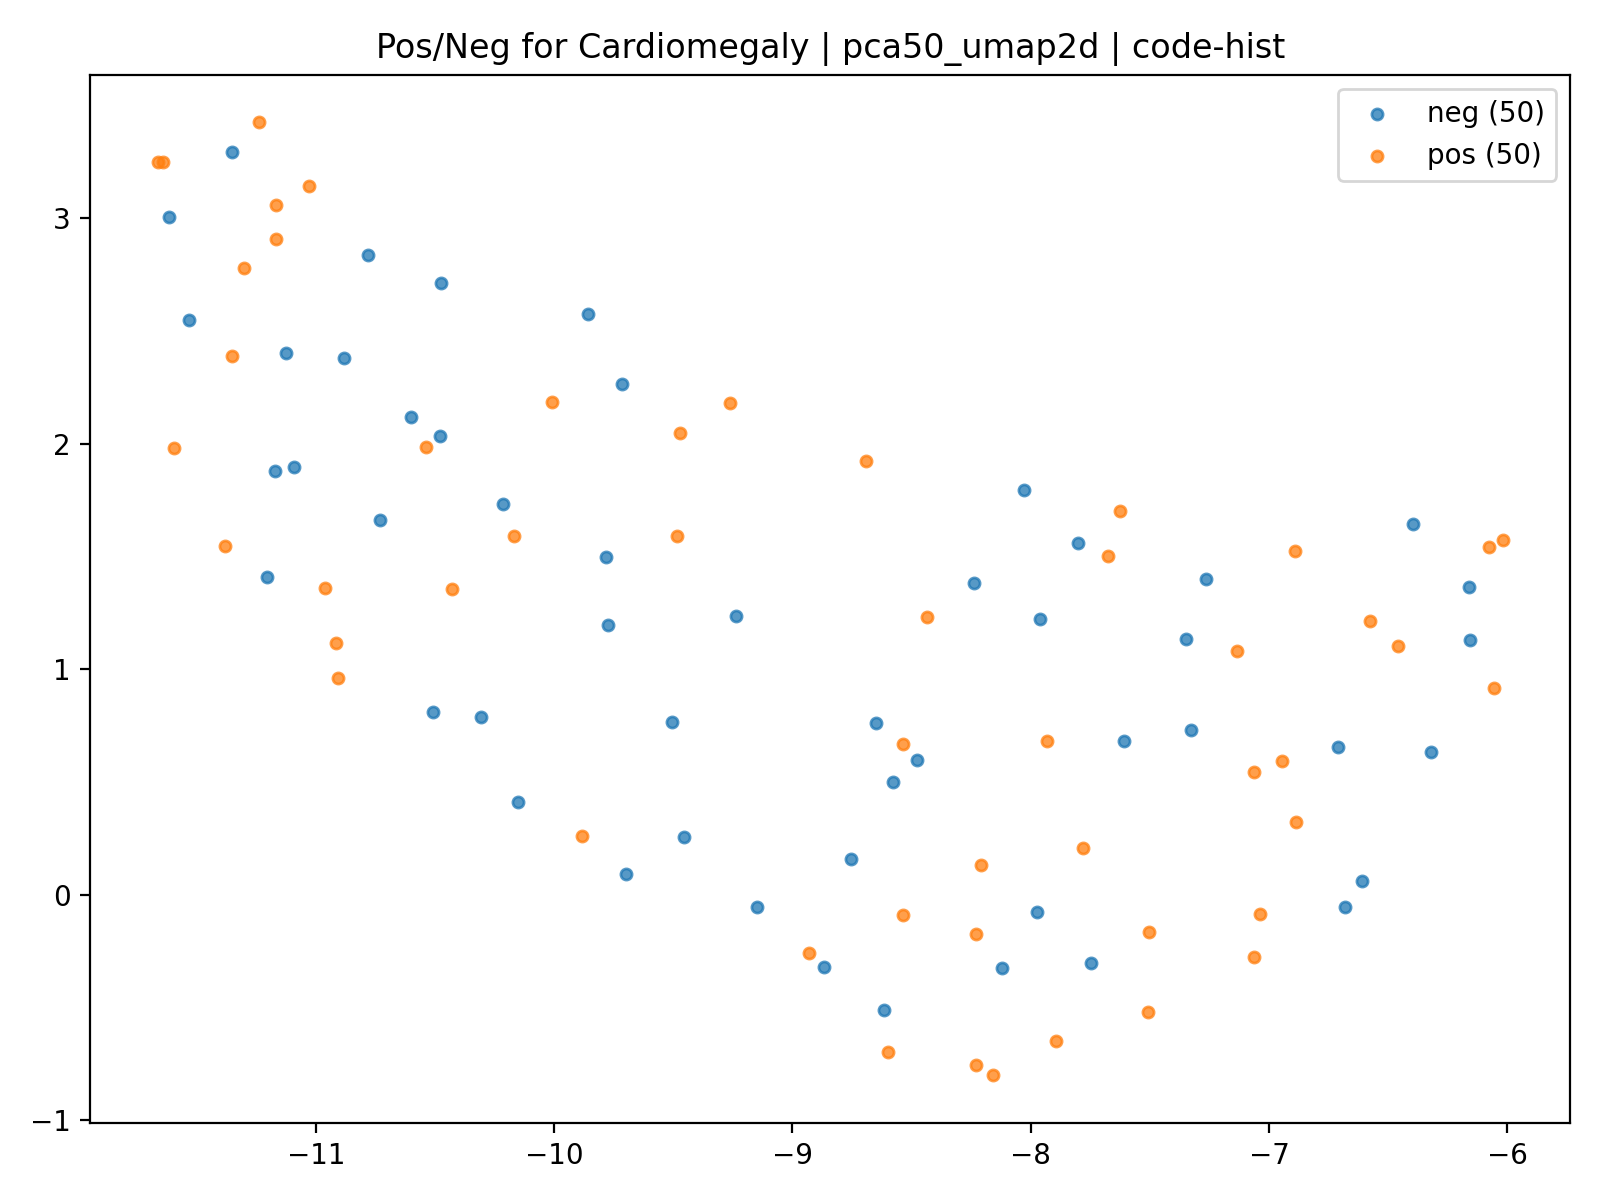
\includegraphics[width=0.8\textwidth]{./images/posneg_Cardiomegaly_pca50_umap2d.png}
    \caption{Latent space visualization of possitive and negative samples of Cardiomegaly class.}
    \label{fig:enter-label}
\end{figure}

From visualization of VAE latents on all pathologies we can see that there is no clear clustering of 
images based on pathologies, this is not true for other datasets like MNIST.  

\section{Image Generation using VAE's}
\begin{figure}[ht]
    \centering

    \begin{subfigure}[t]{0.24\textwidth}
        \centering
        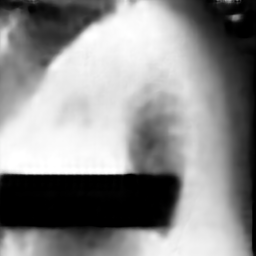
\includegraphics[width=\textwidth]{./images/vqvae_gen/sample_000000.png}
        \caption{}
        \label{fig:vae_gen_1}
    \end{subfigure}
    \hfill
    \begin{subfigure}[t]{0.24\textwidth}
        \centering
        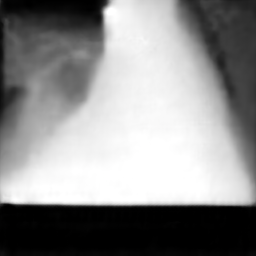
\includegraphics[width=\textwidth]{./images/vqvae_gen/sample_000009.png}
        \caption{}
        \label{fig:vae_gen_2}
    \end{subfigure}
    \hfill
    \begin{subfigure}[t]{0.24\textwidth}
        \centering
        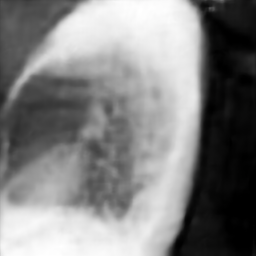
\includegraphics[width=\textwidth]{./images/vqvae_gen/sample_000016.png}
        \caption{}
        \label{fig:vae_gen_3}
    \end{subfigure}
    \hfill
    \begin{subfigure}[t]{0.24\textwidth}
        \centering
        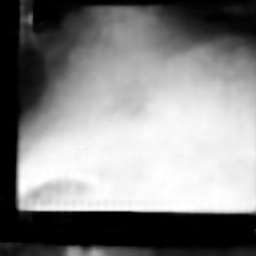
\includegraphics[width=\textwidth]{./images/vqvae_gen/sample_000020.png}
        \caption{}
        \label{fig:vae_gen_4}
    \end{subfigure}

    \caption{Four samples generated by the VAE.}
    \label{fig:vae_gen_four}
\end{figure}





\section{Image Reconstruction using VAE's}

\begin{figure}[ht]
\centering

\setlength{\tabcolsep}{2pt} % reduce horizontal padding between columns
\renewcommand{\arraystretch}{1.0}

\begin{tabular}{cccc}
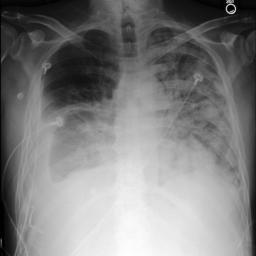
\includegraphics[width=0.24\textwidth]{./images/vqvae_recon/orig/000000_5391944b-b54dc685-7e6f258e-4af54573-0cfe07a5.jpg} &
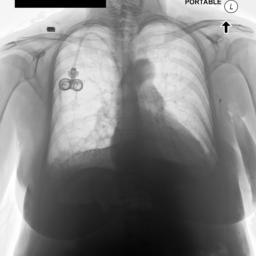
\includegraphics[width=0.24\textwidth]{./images/vqvae_recon/orig/000002_fa22acbe-44e11685-f7500129-c8243d38-b60af2f4.jpg} &
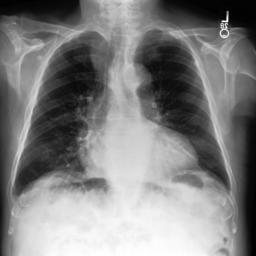
\includegraphics[width=0.24\textwidth]{./images/vqvae_recon/orig/000004_a5c5a35a-bbf9d41e-11d16b10-6369a012-9b46414a.jpg} &
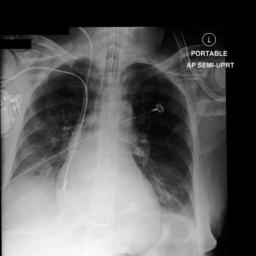
\includegraphics[width=0.24\textwidth]{./images/vqvae_recon/orig/000006_67ba7fde-43d98cc3-cd6efcf2-af65980f-e3daeb17.jpg} \\

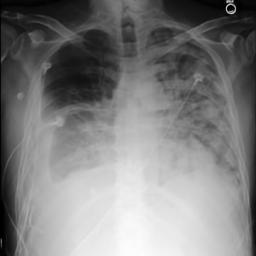
\includegraphics[width=0.24\textwidth]{./images/vqvae_recon/recon/000000_5391944b-b54dc685-7e6f258e-4af54573-0cfe07a5.jpg} &
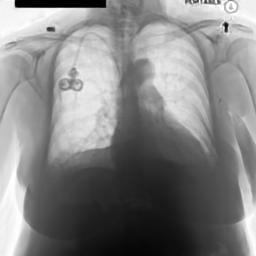
\includegraphics[width=0.24\textwidth]{./images/vqvae_recon/recon/000002_fa22acbe-44e11685-f7500129-c8243d38-b60af2f4.jpg} &
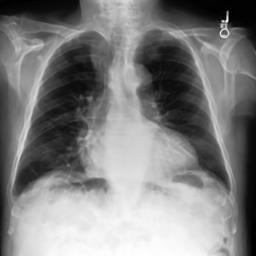
\includegraphics[width=0.24\textwidth]{./images/vqvae_recon/recon/000004_a5c5a35a-bbf9d41e-11d16b10-6369a012-9b46414a.jpg} &
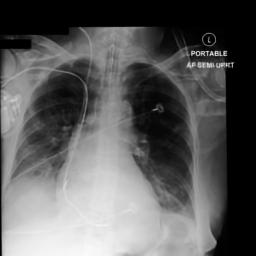
\includegraphics[width=0.24\textwidth]{./images/vqvae_recon/recon/000006_67ba7fde-43d98cc3-cd6efcf2-af65980f-e3daeb17.jpg} \\
\end{tabular}

\caption{Top row: original CXRs. Bottom row: corresponding VAE reconstructions.}
\label{fig:vae_orig_vs_recon_4}
\end{figure}

\section{Validate with FID,LPIPS}
FID of images reconstructed using VAE is 2.9 with just 5000 images, which implies extremely good reconstruction.
LPIPS of images reconstructed using VAE is 0.019 which also implies good reconstruction.

Where as for generation: 


